\documentclass{article}
\usepackage[margin=1in,bottom=1.5in,footskip=1in]{geometry}

\usepackage{multicol}
\usepackage{fancyhdr}
\usepackage{lastpage}
\pagestyle{fancy}
\fancyhf{}
\lfoot{\thepage/10}
\cfoot{
\includegraphics[height=5em]{square_bw}}
\rfoot{Challenge '22}
\renewcommand{\headrulewidth}{0pt}
\renewcommand{\footrulewidth}{0pt}


\usepackage{multicol}

\usepackage{amssymb}
\usepackage{amsmath}

\usepackage{enumerate}

\usepackage{wasysym}


\newcommand{\morseDit}{{\large .}}
\newcommand{\morseDah}{{\large -}}

\usepackage[puttinydots]{braille}


% set font encoding for PDFLaTeX, XeLaTeX, or LuaTeX
\usepackage{ifxetex,ifluatex}
\if\ifxetex T\else\ifluatex T\else F\fi\fi T%
  \usepackage{fontspec}
\else
  \usepackage[T1]{fontenc}
  \usepackage[utf8]{inputenc}
  \usepackage{lmodern}
\fi
\usepackage{tgadventor}
\renewcommand*\familydefault{\sfdefault} %% Only if the base font of the document is to be sans serif

\usepackage{hyperref}
\usepackage{xcolor}
\definecolor{mygray}{gray}{0.8}

\usepackage{tikz}




\newcommand{\clue}[1]{#1}
% UNCOMMENT LINE BELOW TO HIDE CLUES
% \renewcommand{\clue}[1]{}

\newcommand{\puzzleTitle}[1]{
\begin{center}\LARGE\textit{#1}\end{center}
}

\title{Challenge22 draft}
\author{MaPP}


% Enable SageTeX to run SageMath code right inside this LaTeX file.
% http://doc.sagemath.org/html/en/tutorial/sagetex.html
% \usepackage{sagetex}

% Enable PythonTeX to run Python – https://ctan.org/pkg/pythontex
% \usepackage{pythontex}

\begin{document}
%\maketitle

\thispagestyle{empty}
\begin{center}

\includegraphics[width=0.8\linewidth]{banner_bw}

\Large MaPP Challenge '22:

\textit{Terry Kettler and the Mathemagical Mystery}

%Player Book
\end{center}

\vspace{1in}

It finally happened! Although most people get their invitation
when they turn eleven, I, Terry Kettler, finally received my
letter from Professor Ellen Rudin's school for magicians.
Unlike some other schools of magic that you may have read about
or visited in a theme park, Rudin Academy is very real, and
very exclusive.

You see, the letter came with a "Welcome Packet", but it's actually
a collection of puzzles that I'll need to solve in order to be
accepted. Of course, by "me" I really mean "we" - I hear you're
pretty great at solving puzzles, and I may have put off my application
until the last minute...

I've made you a copy of this welcome packet. It won't
make much sense by itself, but I'll send you messages using the
ClueKeeper app that will help your team solve the enigmata hidden within
these pages. You'll be finding several "magic codes"
and "magic words"; submit them using your ClueKeeper app so I can
include them in my application.
If you can solve enough of these puzzles, they'll have to let me join their
school, right?



\begin{center}

\end{center}

\vfill

{\footnotesize PDF last updated: \today}

\newpage


\puzzleTitle{Our Mentoring Program}

\vfill

\begin{center}
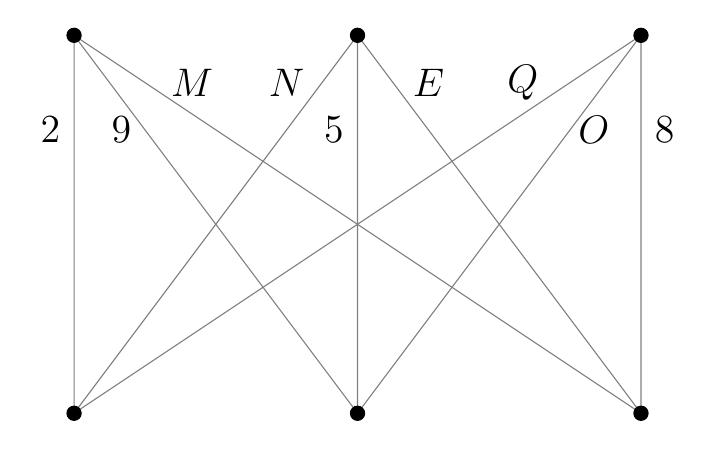
\begin{tikzpicture}[scale=1.2]
\draw[gray] (0,0) -- (0,4)--(3,0)--(3,4)--(6,0)--(6,4)--cycle;
\draw[gray] (0,0)--(3,4);
\draw[gray] (0,4)--(6,0);
\draw[gray] (3,0)--(6,4);

\draw[fill=black] (0,4) circle (0.075);
\draw[fill=black] (0,0) circle (0.075);
\draw[fill=black] (3,0) circle (0.075);
\draw[fill=black] (3,4) circle (0.075);
\draw[fill=black] (6,0) circle (0.075);
\draw[fill=black] (6,4) circle (0.075);
{\Large

\node at (1.25,3.5) {$M$};
\node at (2.25,3.5) {$N$};
\node at (3.75,3.5) {$E$};
\node at (4.75,3.5) {$Q$};
\node at (-.25,3) {$2$};
\node at (.5,3) {$9$};
\node at (2.75,3) {$5$};
\node at (5.5,3) {$O$};
\node at (6.25,3) {$8$};
}


\end{tikzpicture}


\vfill
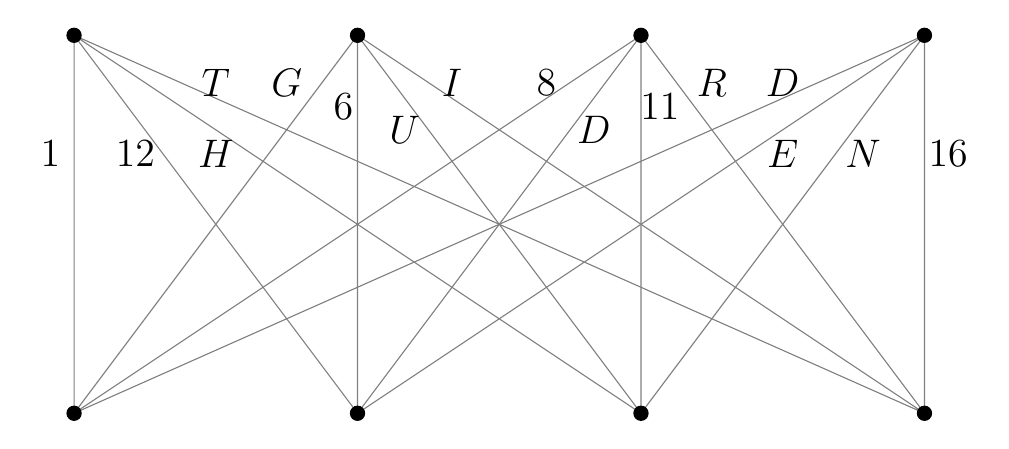
\begin{tikzpicture}[scale=1.2]
%\draw[step=1,black!20] (0,0) grid (9,4);
\draw[gray] (0,0) -- (0,4)--(3,0)--(3,4)--(6,0)--(6,4)--(9,0)--(9,4)--cycle;
\draw[gray] (0,0)--(3,4)--(9,0)--(0,4)--(6,0)--(9,4)--(3,0)--(6,4)--cycle;

{\Large
\node at (1.5,3.5) {$T$};
\node at (2.25,3.5) {$G$};
\node at (4,3.5) {$I$};
\node at (5,3.5) {$8$};
\node at (6.75,3.5) {$R$};
\node at (7.5,3.5) {$D$};
\node at (2.85,3.25) {$6$};
\node at (3.5,3) {$U$};
\node at (5.5,3) {$D$};
\node at (6.2,3.25) {$11$};
\node at (-.25,2.75) {$1$};
\node at (.65,2.75) {$12$};
\node at (1.5,2.75) {$H$};
\node at (7.5,2.75) {$E$};
\node at (8.35,2.75) {$N$};
\node at (9.25,2.75) {$16$};
}

\draw[fill=black] (0,4) circle (0.075);
\draw[fill=black] (0,0) circle (0.075);
\draw[fill=black] (3,0) circle (0.075);
\draw[fill=black] (3,4) circle (0.075);
\draw[fill=black] (6,0) circle (0.075);
\draw[fill=black] (6,4) circle (0.075);
\draw[fill=black] (9,4) circle (0.075);
\draw[fill=black] (9,0) circle (0.075);
\end{tikzpicture}

\vfill
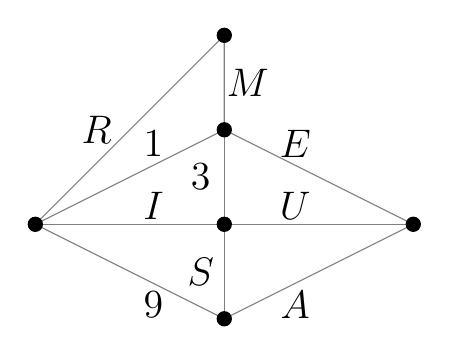
\begin{tikzpicture}[scale=1.2]
%\draw[step=1,black!20] (0,-1) grid (4,2);
\draw[gray] (0,0) -- (2,1)--(4,0)--(2,-1)--cycle;
\draw[gray] (0,0) -- (2,2)--(2,1);
\draw[gray] (0,0)--(4,0);
\draw[gray] (2,1)--(2,-1);

\draw[fill=black] (0,0) circle (0.075);
\draw[fill=black] (2,-1) circle (0.075);
\draw[fill=black] (2,0) circle (0.075);
\draw[fill=black] (2,1) circle (0.075);
\draw[fill=black] (2,2) circle (0.075);
\draw[fill=black] (4,0) circle (0.075);

{\Large
\node at (.65,1) {$R$};
\node at (2.25,1.5) {$M$};
\node at (1.25,.85) {$1$};
\node at (2.75,.85) {$E$};
\node at (1.75,.5) {$3$};
\node at (1.25,.2) {$I$};
\node at (2.75,.2) {$U$};
\node at (1.25,-.85) {$9$};
\node at (2.75,-.85) {$A$};
\node at (1.75,-.5) {$S$};
}

\end{tikzpicture}
\end{center}
\vspace*{2cm}
\begin{center}
\includegraphics[width=\linewidth]{labelings/key.png}
\end{center}
\newpage




\puzzleTitle{Our Tuition Schedule}

\vfill

\begin{center}
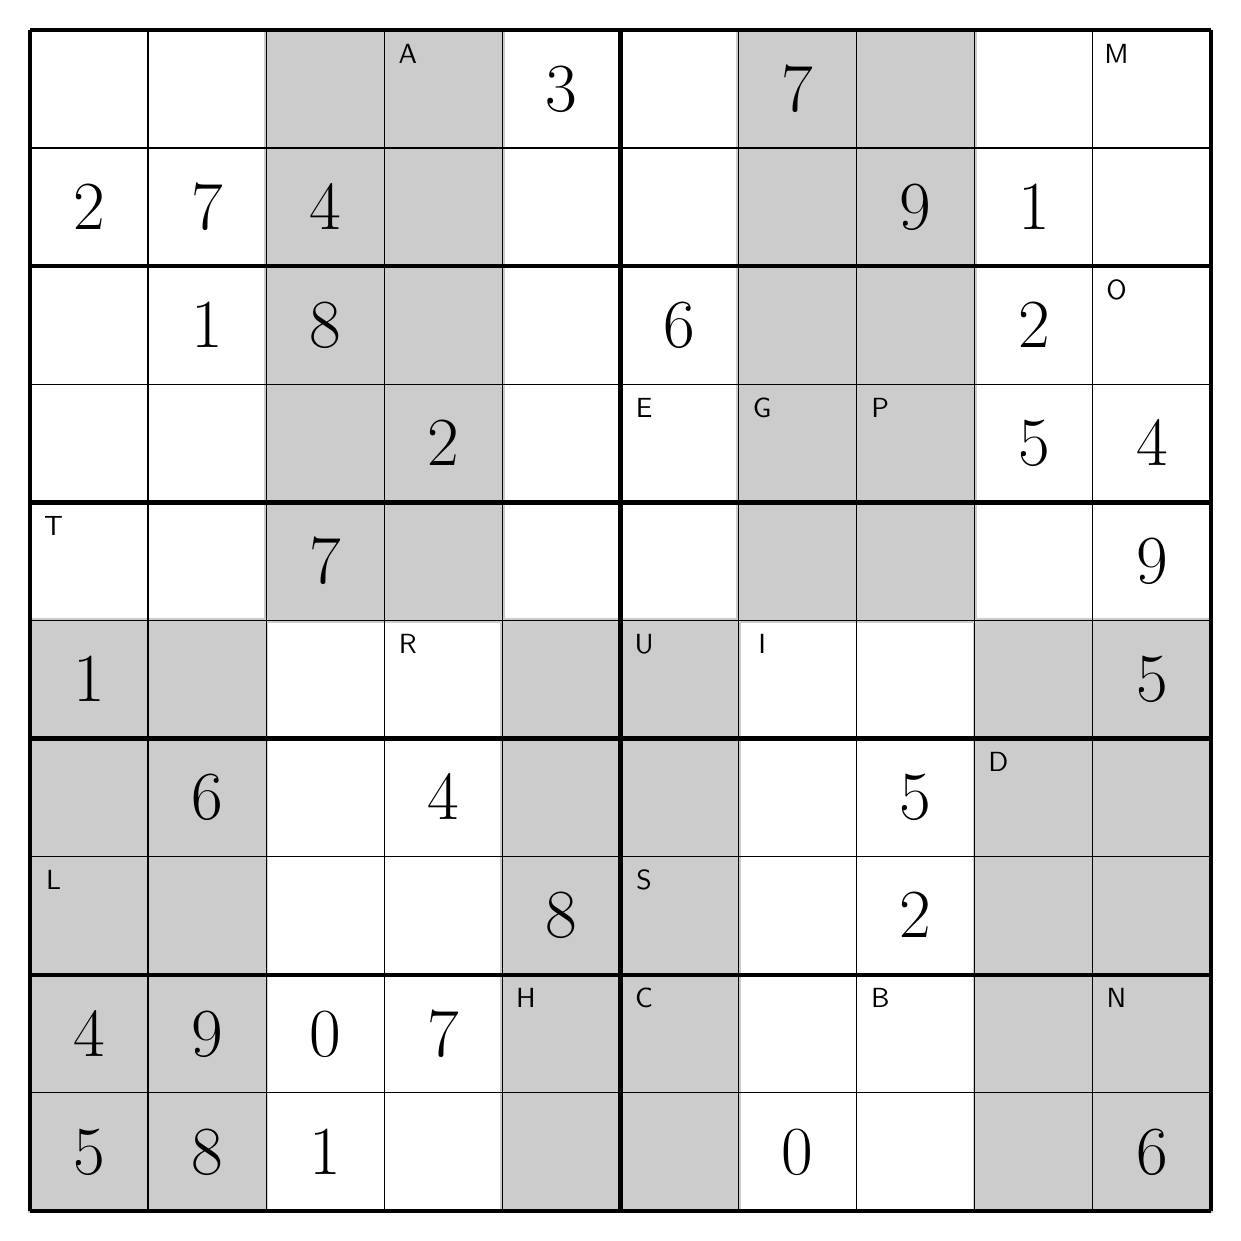
\begin{tikzpicture}[scale=1.5]
\draw[fill=black!05,ultra thick,color=black!20](0,0) rectangle (2,5);
\draw[fill=black!05,ultra thick,color=black!20](2,5) rectangle (4,10);
\draw[fill=black!05,ultra thick,color=black!20](4,0) rectangle (6,5);
\draw[fill=black!05,ultra thick,color=black!20](6,5) rectangle (8,10);
\draw[fill=black!05,ultra thick,color=black!20](8,0) rectangle (10,5);
\draw[step=10,ultra thick](0,0)grid(10,10);

 
\draw(0,0)grid(10,10);
%\draw(3,0)grid(3,10);
%\draw(5,0)grid(5,10);
%\draw(7,0)grid(7,10);
%\draw(9,0)grid(9,10);
% 
%\draw(0,1)grid(10,1);
%\draw(0,3)grid(10,3);
%% \draw(0,5)grid(10,5);
%\draw(0,7)grid(10,7);
%\draw(0,9)grid(10,9);
 
\draw[ultra thick](0,2)grid(10,2);
\draw[ultra thick](0,4)grid(10,4);
\draw[ultra thick](0,6)grid(10,6);
\draw[ultra thick](0,8)grid(10,8);
\draw[ultra thick](5,0)grid(5,10);
 
%\draw[loosely dashed](2,0)grid(2,10);
%\draw[loosely dashed](4,0) to (4,10);
%\draw[loosely dashed](6,0)grid(6,10);
%\draw[loosely dashed](8,0)grid(8,10);
%\draw[loosely dashed](0,5) to (10,5);
 
 {\Huge
\foreach\x[count=\i] in{ , , , ,3 , ,7,,,}{\node at(\i-0.5,9.5){$\x$};};
\foreach\x[count=\i] in{ 2,7,4,, , , ,9,1, }{\node at(\i-0.5,8.5){$\x$};};
\foreach\x[count=\i] in{ ,1,8, ,,6,, ,2,}{\node at(\i-0.5,7.5){$\x$};};
\foreach\x[count=\i] in{ ,,,2 , ,, , ,5 ,4}{\node at(\i-0.5,6.5){$\x$};};
\foreach\x[count=\i] in{ , ,7 , , , ,, , ,9 }{\node at(\i-0.5,5.5){$\x$};};
\foreach\x[count=\i] in{ 1,, ,, , ,,, ,5 }{\node at(\i-0.5,4.5){$\x$};};
\foreach\x[count=\i] in{ ,6 ,,4,,,, 5, , }{\node at(\i-0.5,3.5){$\x$};};
\foreach\x[count=\i] in{ , ,, ,8, , ,2, , }{\node at(\i-0.5,2.5){$\x$};};
\foreach\x[count=\i] in{ 4, 9,0 ,7 , , ,,, , }{\node at(\i-0.5,1.5){$\x$};};
\foreach\x[count=\i] in{ 5,8 ,1, , , , 0, , ,6 }{\node at(\i-0.5,0.5){$\x$};};
}
 {
\foreach\x[count=\i] in{ , , ,A , , ,,,,M}{\node at(\i-0.8,9.8){\x};};
\foreach\x[count=\i] in{ ,,,, , , ,,, }{\node at(\i-0.8,8.8){\x};};
\foreach\x[count=\i] in{ ,,, ,,,, ,,O}{\node at(\i-0.8,7.8){\x};};
\foreach\x[count=\i] in{ ,,, , ,E, G,P , ,}{\node at(\i-0.8,6.8){\x};};
\foreach\x[count=\i] in{ T, , , , , ,, , , }{\node at(\i-0.8,5.8){\x};};
\foreach\x[count=\i] in{ ,, ,R, ,U ,I,, , }{\node at(\i-0.8,4.8){\x};};
\foreach\x[count=\i] in{ , ,,,,,, , D, }{\node at(\i-0.8,3.8){\x};};
\foreach\x[count=\i] in{ L, ,, ,,S , ,, , }{\node at(\i-0.8,2.8){\x};};
\foreach\x[count=\i] in{ , , , ,H ,C ,,B, ,N }{\node at(\i-0.8,1.8){\x};};
\foreach\x[count=\i] in{ , ,, , , , , , , }{\node at(\i-0.8,0.8){\x};};
}
\end{tikzpicture}\end{center}

\vfill

\newpage





\newpage

\puzzleTitle{Our Curriculum}

\vfill

\begin{center}
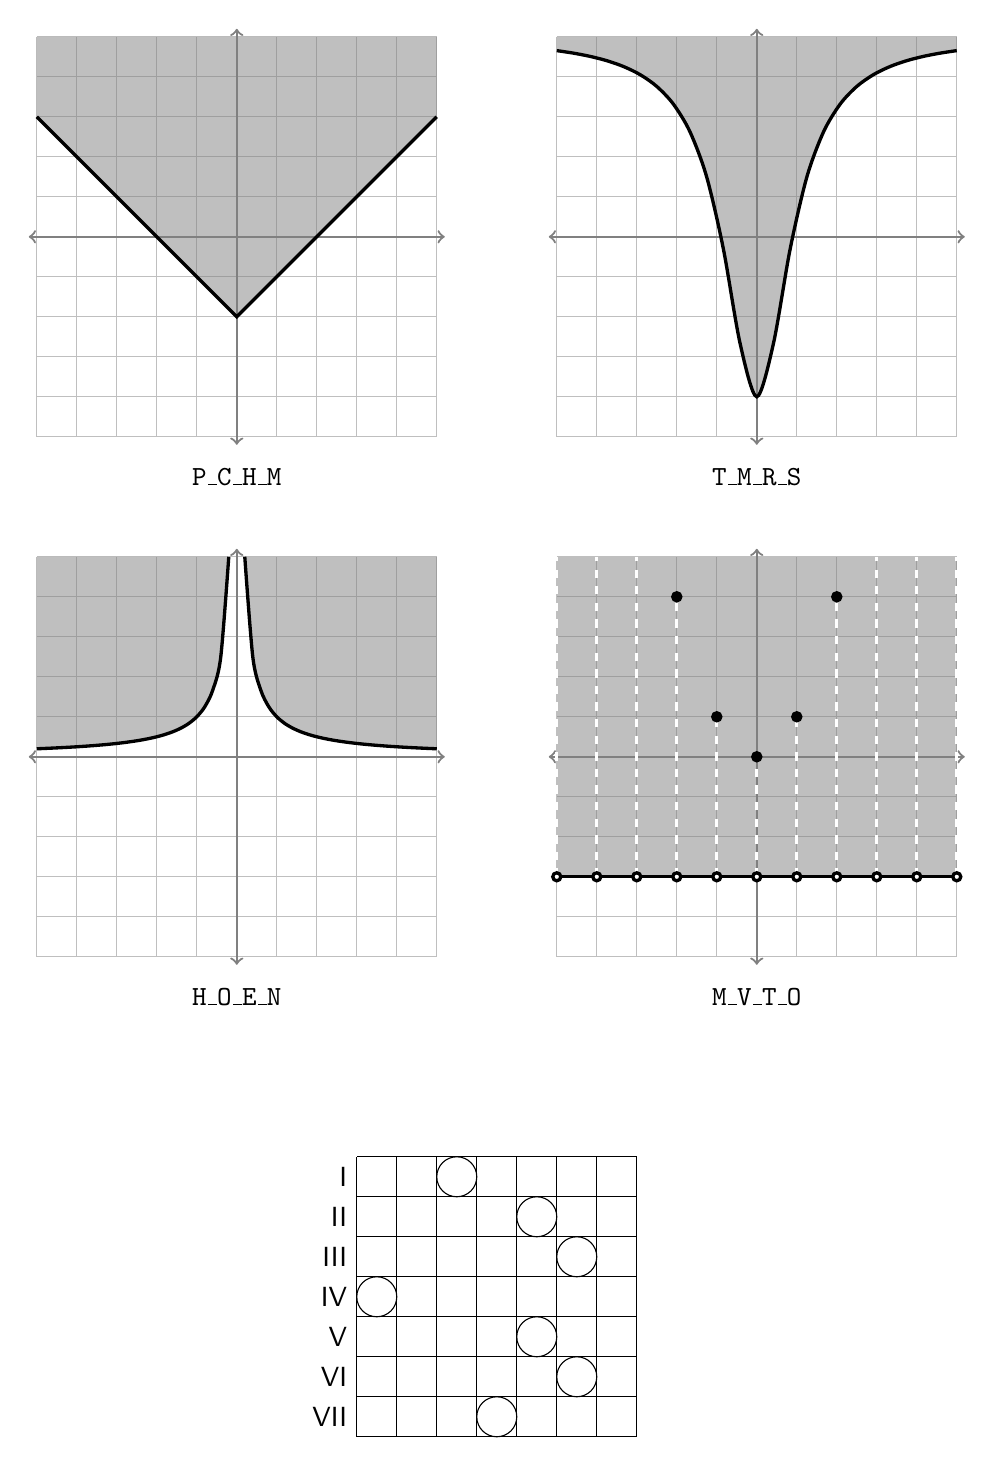
\begin{tikzpicture}[x=0.2in,y=0.2in]
  \begin{scope}[shift={(0,0)}]
  \draw[gray!50, thin, step=1] (-5,-5) grid (5,5);
  \draw[gray,thick,<->] (-5.2,0) -- (5.2,0);
  \draw[gray,thick,<->] (0,-5.2) -- (0,5.2);
  \fill[fill=gray,opacity=0.5]  (-5,3) -- (-5,5) -- (5,5) -- (5,3) -- (0,-2); 
  \draw[black,very thick]  (-5,3) -- (0,-2) -- (5,3); 
  \node at (0,-6) {\texttt{P\_C\_H\_M}};%PACUHUM
  \end{scope}

  \begin{scope}[shift={(13,0)}]
  \draw[gray!50, thin, step=1] (-5,-5) grid (5,5);
  \draw[gray,thick,<->] (-5.2,0) -- (5.2,0);
  \draw[gray,thick,<->] (0,-5.2) -- (0,5.2);
  \fill[gray,opacity=0.5]   plot[smooth,domain=-5:5] (\x, {(5*\x*\x-4)/(\x*\x+1)})
    -- (5,5) -- (-5,5);
  \draw[black,very thick]   plot[smooth,domain=-5:5] (\x, {(5*\x*\x-4)/(\x*\x+1)});
  \node at (0,-6) {\texttt{T\_M\_R\_S}};%TIMARUS
  \end{scope}

  \begin{scope}[shift={(0,-13)}]
  \draw[gray!50, thin, step=1] (-5,-5) grid (5,5);
  \draw[gray,thick,<->] (-5.2,0) -- (5.2,0);
  \draw[gray,thick,<->] (0,-5.2) -- (0,5.2);
  \fill[gray,opacity=0.5]   plot[smooth,domain=-5:-0.2] (\x, {-1/(\x)}) -- (-5,5);
  \draw[black,very thick]   plot[smooth,domain=-5:-0.2] (\x, {-1/(\x)});
  \fill[gray,opacity=0.5]   plot[smooth,domain=0.2:5] (\x, {1/(\x)}) -- (5,5);
  \draw[black,very thick]   plot[smooth,domain=0.2:5] (\x, {1/(\x)});
  \node at (0,-6) {\texttt{H\_O\_E\_N}};%HOLFEIN
  \end{scope}

  \begin{scope}[shift={(13,-13)}]
  \draw[gray!50, thin, step=1] (-5,-5) grid (5,5);
  \draw[gray,thick,<->] (-5.2,0) -- (5.2,0);
  \draw[gray,thick,<->] (0,-5.2) -- (0,5.2);
  \fill[gray,opacity=0.5] (-5,-3) rectangle (5,5);
  \draw[black,very thick] (-5,-3) -- (5,-3);
  \foreach \n in {-2,-1,0,1,2} {
    \draw[very thick,white,dashed] (\n,-3) -- (\n,\n*\n);
    \draw[very thick,fill=white] (\n,-3) circle (0.1);
    \draw[very thick,fill=black] (\n,\n*\n) circle (0.1);
  }
  \foreach \n in {-5,-4,-3,3,4,5} {
    \draw[very thick,white,dashed] (\n,-3) -- (\n,5);
    \draw[very thick,fill=white] (\n,-3) circle (0.1);
  }
  \node at (0,-6) {\texttt{M\_V\_T\_O}};%MAVETRO
  \end{scope}

  \begin{scope}[shift={(3,-30)}]
  \draw[step=1] (0,0) grid (7,7);
  \node[anchor=east] at (0,0.5) {VII};
  \node[anchor=east] at (0,1.5) {VI};
  \node[anchor=east] at (0,2.5) {V};
  \node[anchor=east] at (0,3.5) {IV};
  \node[anchor=east] at (0,4.5) {III};
  \node[anchor=east] at (0,5.5) {II};
  \node[anchor=east] at (0,6.5) {I};
  \draw (2.5,6.5) circle (0.5);
  \draw (4.5,5.5) circle (0.5);
  \draw (5.5,4.5) circle (0.5);
  \draw (0.5,3.5) circle (0.5);
  \draw (4.5,2.5) circle (0.5);
  \draw (5.5,1.5) circle (0.5);
  \draw (3.5,0.5) circle (0.5);
  \end{scope}
\end{tikzpicture}
\end{center}

\vfill

\newpage




\puzzleTitle{Our Placement Exam}

\vfill

{\huge
\[8\div 4\times 3+1\times 9-7\]\vfill
\[7\times 4\div 9-9-6\div 3\]\vfill
\[3+5\div 4-2+5-2\]\vfill
\[9-4\times 3-3+4\div 2\]\vfill
\[9\div 3+2\times 1+5-3\]\vfill
\[5\div 3+7-6-5-4\]\vfill
\[5+3\div 2\times 6+2\div 2\]\vfill
\[2+1-9-2+3\times 4\]\vfill
\[9-4\times 2+8\div 4-2\]\vfill
}

\vfill

\begin{center}\LARGE
\(1\)\hfill
\(3\)\hfill
\(8\)\hfill
\(8\)\hfill
\(8\)\hfill
\(13\)\hfill
\(14\)\hfill
\(14\)\hfill
\(15\)
\end{center}



\vfill

\newpage


\puzzleTitle{Our Night Sky}

\vfill

\begin{center}\Large
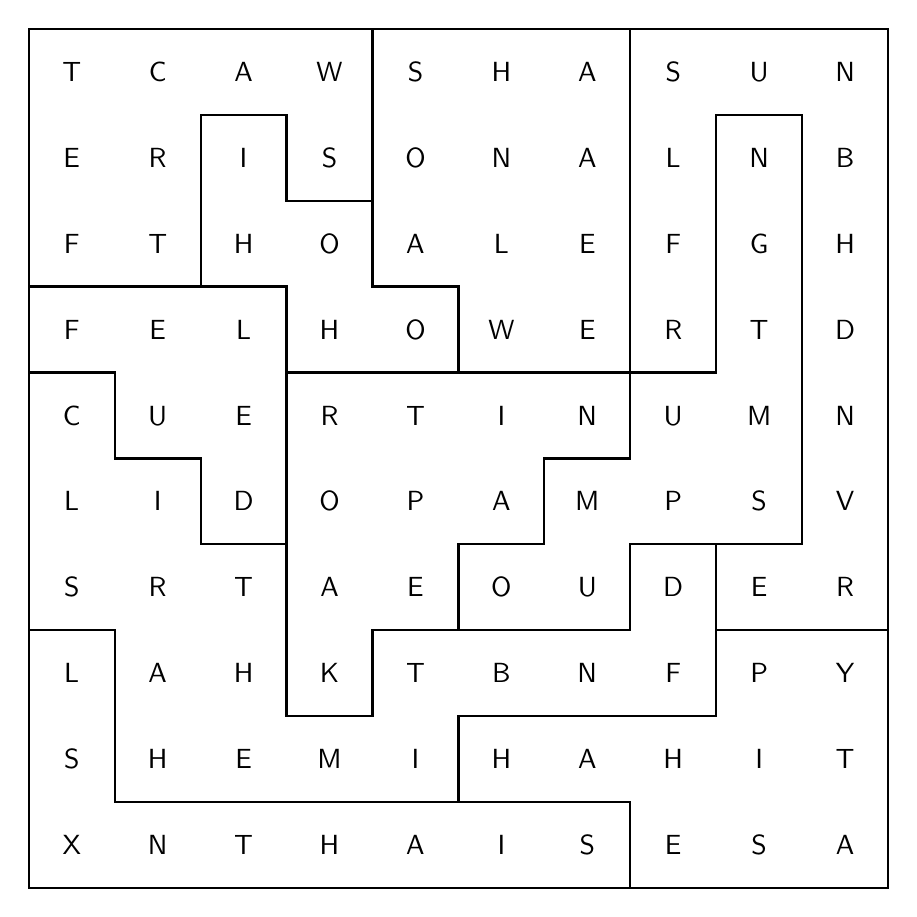
\begin{tikzpicture}[x=0.09\linewidth,y=0.09\linewidth]
\draw[thick,black] (0,0) rectangle (10,10);
\draw[thick,black] (0,3) -- (1,3) -- (1,1) -- (7,1) -- (7,0);
\draw[thick,black] (0,6) -- (1,6) -- (1,5) -- (2,5) -- (2,4) --
                   (3,4) -- (3,2) -- (4,2) -- (4,3) -- (7,3) --
                   (7,4) -- (8,4) -- (8,2) -- (5,2) -- (5,1);
\draw[thick,black] (8,3) -- (10,3);
\draw[thick,black] (8,4) -- (9,4) -- (9,9) -- (8,9) -- (8,6) --
                   (7,6) -- (7,10);
\draw[thick,black] (7,6) -- (7,5) -- (6,5) -- (6,4) -- (5,4) --
                   (5,3);
\draw[thick,black] (3,4) -- (3,6) -- (7,6);
\draw[thick,black] (3,6) -- (3,7) -- (0,7);
\draw[thick,black] (2,7) -- (2,9) -- (3,9) -- (3,8) -- (4,8) --
                   (4,7) -- (5,7) -- (5,6);
\draw[thick,black] (4,8) -- (4,10);

\foreach\x[count=\i from 0] in {T,C,A,W,S,H,A,S,U,N}{\node at(\i.5,9.5){\x};};
\foreach\x[count=\i from 0] in {E,R,I,S,O,N,A,L,N,B}{\node at(\i.5,8.5){\x};};
\foreach\x[count=\i from 0] in {F,T,H,O,A,L,E,F,G,H}{\node at(\i.5,7.5){\x};};
\foreach\x[count=\i from 0] in {F,E,L,H,O,W,E,R,T,D}{\node at(\i.5,6.5){\x};};
\foreach\x[count=\i from 0] in {C,U,E,R,T,I,N,U,M,N}{\node at(\i.5,5.5){\x};};
\foreach\x[count=\i from 0] in {L,I,D,O,P,A,M,P,S,V}{\node at(\i.5,4.5){\x};};
\foreach\x[count=\i from 0] in {S,R,T,A,E,O,U,D,E,R}{\node at(\i.5,3.5){\x};};
\foreach\x[count=\i from 0] in {L,A,H,K,T,B,N,F,P,Y}{\node at(\i.5,2.5){\x};};
\foreach\x[count=\i from 0] in {S,H,E,M,I,H,A,H,I,T}{\node at(\i.5,1.5){\x};};
\foreach\x[count=\i from 0] in {X,N,T,H,A,I,S,E,S,A}{\node at(\i.5,0.5){\x};};
\end{tikzpicture}
\end{center}

\vfill

\newpage



\newpage

\puzzleTitle{Our Calendar}

\vfill

\newcommand{\SymbMon}[1]{\begin{tikzpicture}[scale=#1]
\fill [white] (-1,-1) rectangle (1,1);
\draw [thick,domain=90:270] plot ({cos(\x)}, {sin(\x)});
\draw [thick,domain=135:225] plot ({1+1.41*cos(\x)}, {1.41*sin(\x)});
\end{tikzpicture}}
\newcommand{\SymbTue}[1]{\begin{tikzpicture}[scale=#1]
\fill [white] (-1,-1) rectangle (1,1);
\draw [thick] (0,0) -- (1.1,1.1) -- (0.7,1.1);
\draw [thick] (0,0) -- (1.1,1.1) -- (1.1,0.7);
\draw [fill=white,thick,domain=0:360] plot ({0.9*cos(\x)}, {0.9*sin(\x)});
\end{tikzpicture}}
\newcommand{\SymbWed}[1]{\begin{tikzpicture}[scale=#1]
\fill [white] (-1,-1) rectangle (1,1);
\draw [thick] (0,-1) -- (0,-0.5);
\draw [thick] (-0.25,-0.75) -- (0.25,-0.75);
\draw [fill=white,thick,domain=0:360] plot ({0.5*cos(\x)}, {0.5*sin(\x)});
\draw [fill=white,thick,domain=0:-180] plot ({0.5*cos(\x)}, {1+0.5*sin(\x)});
\end{tikzpicture}}
\newcommand{\SymbThu}[1]{\begin{tikzpicture}[scale=#1]
\fill [white] (-0.75,-0.5) rectangle (1.25,1.5);
\draw [thick] (0,0) -- (1,0);
\draw [thick] (0.5,-0.5) -- (0.5,0.5);
\draw [fill=white,thick,domain=-90:180] plot ({0.25*cos(\x)}, {0.75+0.75*sin(\x)});
\end{tikzpicture}}
\newcommand{\SymbFri}[1]{\begin{tikzpicture}[scale=#1]
\fill [white] (-1,-1) rectangle (1,1);
\draw [thick] (0,-1) -- (0,-0.5);
\draw [thick] (-0.25,-0.75) -- (0.25,-0.75);
\draw [fill=white,thick,domain=0:360] plot ({0.75*cos(\x)}, {0.25+0.75*sin(\x)});
\end{tikzpicture}}
\newcommand{\SymbSat}[1]{\begin{tikzpicture}[scale=#1]
\fill [white] (-1,-1) rectangle (1,1);
\draw [thick] (-0.5,-0.75) -- (-0.5,1);
\draw [thick] (-0.75,0.75) -- (-0.25,0.75);
\draw [fill=white,thick,domain=180:-90] plot ({0.5*cos(\x)}, {0.5*sin(\x)});
\draw [fill=white,thick,domain=90:270] plot ({0.25*cos(\x)}, {-0.75+0.25*sin(\x)});
\end{tikzpicture}}
\newcommand{\SymbSun}[1]{\begin{tikzpicture}[scale=#1]
\fill [white] (-1,-1) rectangle (1,1);
\draw [thick,domain=0:360] plot ({cos(\x)}, {sin(\x)});
\draw [fill,thick,domain=0:360] plot ({0.1*cos(\x)}, {0.1*sin(\x)});
\end{tikzpicture}}
\newcommand{\SymbMag}[1]{\begin{tikzpicture}[scale=#1]
\fill [white] (-1,-1) rectangle (1,1);
\draw [thick] (-1,0.8) -- (-0.8,1) -- (1,-0.8) -- (0.8,-1) -- (-1,0.8);
\draw [thick,fill=white] (-0.7,-0.7) rectangle (0.7,0.7);
\end{tikzpicture}}

\begin{center}\Huge
\begin{tabular}{cccccccc}
\SymbMon{0.6} & \SymbTue{0.6} & \SymbWed{0.6} & \SymbThu{0.6} &
\SymbFri{0.6} & \SymbSat{0.6} & \SymbSun{0.6} & \SymbMag{0.6} \\\hline
1 & 2 & 3 & 4 & 5 & 6 & 7 & \\
8 & 9 & 10 & 11 & 12 & 13 & 14 & \\
15 & 16 & 17 & 18 & 19 & 20 & 21 & \\
22 & 23 & 24 & 25 & 26 & 27 & 28 & (29)
\end{tabular}

\end{center}

\vfill

\begin{center}\Large
FUSION: 443 days with the 261st day on a Magday

HERESY: 414 days with the 355th day on a Magday

LIVING: 430 days with the 223rd day on a Magday

MEMORY: 410 days with the 306th day on a Magday

MYTHOS: 425 days with the 114th day on a Magday

WISHES: 406 days with the 155th day on a Magday
\end{center}


\vfill

\newpage


\puzzleTitle{Our Seal}

\vfill

\newcommand{\nonosize}[1]{\textcolor{black!30}{#1}}
\begin{center}
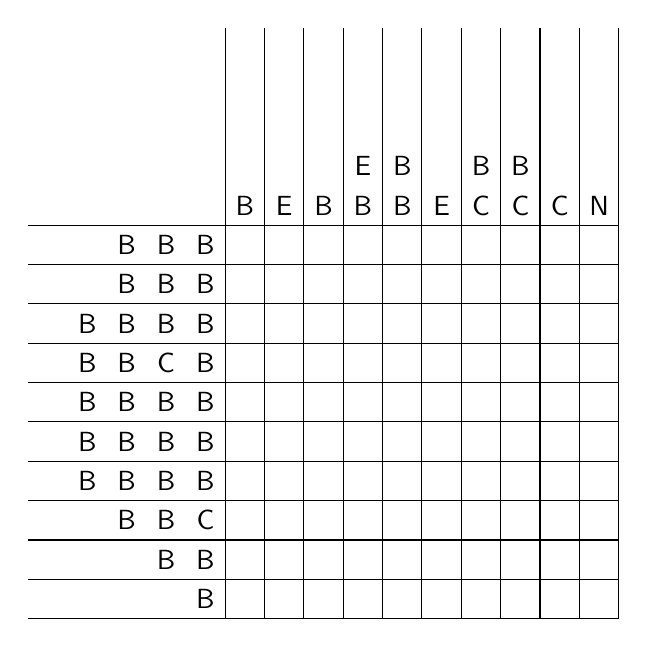
\begin{tikzpicture}[scale=0.5]
%\node at (-2.5,12.5) {Virgo};
   
    \foreach \n in {0,...,10}{
        \draw (-5,\n)--(10,\n);
        \draw (\n,0)--(\n,15);
    }
   
    %Horizontal Clues (backwards in source)
    \foreach[count=\n] \x in {B,B,B}{\node at ({0.5-\n},9.5) {\nonosize{\x}}; }
    \foreach[count=\n] \x in {B,B,B}{\node at ({0.5-\n},8.5) {\nonosize{\x}}; }
    \foreach[count=\n] \x in {B,B,B,B}{\node at ({0.5-\n},7.5) {\nonosize{\x}}; }
    \foreach[count=\n] \x in {B,C,B,B}{\node at ({0.5-\n},6.5) {\nonosize{\x}}; }
    \foreach[count=\n] \x in {B,B,B,B}{\node at ({0.5-\n},5.5) {\nonosize{\x}}; }
    \foreach[count=\n] \x in {B,B,B,B}{\node at ({0.5-\n},4.5) {\nonosize{\x}}; }
    \foreach[count=\n] \x in {B,B,B,B}{\node at ({0.5-\n},3.5) {\nonosize{\x}}; }
    \foreach[count=\n] \x in {C,B,B}{\node at ({0.5-\n},2.5) {\nonosize{\x}}; }
    \foreach[count=\n] \x in {B,B}{\node at ({0.5-\n},1.5) {\nonosize{\x}}; }
    \foreach[count=\n] \x in {B}{\node at ({0.5-\n},0.5) {\nonosize{\x}}; }
   
    %Vertical Clues (backwards in source)
    \foreach[count=\n] \x in {B}{\node at (0.5,{9.5+\n}) {\nonosize{\x}}; }
    \foreach[count=\n] \x in {E}{\node at (1.5,{9.5+\n}) {\nonosize{\x}}; }
    \foreach[count=\n] \x in {B}{\node at (2.5,{9.5+\n}) {\nonosize{\x}}; }
    \foreach[count=\n] \x in {B,E}{\node at (3.5,{9.5+\n}) {\nonosize{\x}}; }
    \foreach[count=\n] \x in {B,B}{\node at (4.5,{9.5+\n}) {\nonosize{\x}}; }
    \foreach[count=\n] \x in {E}{\node at (5.5,{9.5+\n}) {\nonosize{\x}}; }
    \foreach[count=\n] \x in {C,B}{\node at (6.5,{9.5+\n}) {\nonosize{\x}}; }
    \foreach[count=\n] \x in {C,B}{\node at (7.5,{9.5+\n}) {\nonosize{\x}}; }
    \foreach[count=\n] \x in {C}{\node at (8.5,{9.5+\n}) {\nonosize{\x}}; }
    \foreach[count=\n] \x in {N}{\node at (9.5,{9.5+\n}) {\nonosize{\x}}; }
\end{tikzpicture}

\end{center}

\vfill

\begin{center}
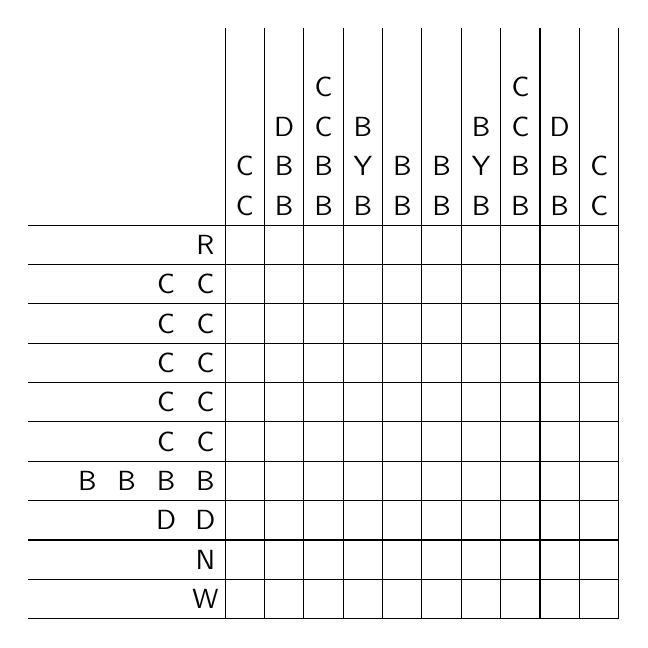
\begin{tikzpicture}[scale=0.5]
%\node at (-2.5,12.5) {Libra};
   
    \foreach \n in {0,...,10}{
        \draw (-5,\n)--(10,\n);
        \draw (\n,0)--(\n,15);
    }
   
    %Horizontal Clues (backwards in source)
    \foreach[count=\n] \x in {R}{\node at ({0.5-\n},9.5) {\nonosize{\x}}; }
    \foreach[count=\n] \x in {C,C}{\node at ({0.5-\n},8.5) {\nonosize{\x}}; }
    \foreach[count=\n] \x in {C,C}{\node at ({0.5-\n},7.5) {\nonosize{\x}}; }
    \foreach[count=\n] \x in {C,C}{\node at ({0.5-\n},6.5) {\nonosize{\x}}; }
    \foreach[count=\n] \x in {C,C}{\node at ({0.5-\n},5.5) {\nonosize{\x}}; }
    \foreach[count=\n] \x in {C,C}{\node at ({0.5-\n},4.5) {\nonosize{\x}}; }
    \foreach[count=\n] \x in {B,B,B,B}{\node at ({0.5-\n},3.5) {\nonosize{\x}}; }
    \foreach[count=\n] \x in {D,D}{\node at ({0.5-\n},2.5) {\nonosize{\x}}; }
    \foreach[count=\n] \x in {N}{\node at ({0.5-\n},1.5) {\nonosize{\x}}; }
    \foreach[count=\n] \x in {W}{\node at ({0.5-\n},0.5) {\nonosize{\x}}; }
   
    %Vertical Clues (backwards in source)
    \foreach[count=\n] \x in {C,C}{\node at (0.5,{9.5+\n}) {\nonosize{\x}}; }
    \foreach[count=\n] \x in {B,B,D}{\node at (1.5,{9.5+\n}) {\nonosize{\x}}; }
    \foreach[count=\n] \x in {B,B,C,C}{\node at (2.5,{9.5+\n}) {\nonosize{\x}}; }
    \foreach[count=\n] \x in {B,Y,B}{\node at (3.5,{9.5+\n}) {\nonosize{\x}}; }
    \foreach[count=\n] \x in {B,B}{\node at (4.5,{9.5+\n}) {\nonosize{\x}}; }
    \foreach[count=\n] \x in {B,B}{\node at (5.5,{9.5+\n}) {\nonosize{\x}}; }
    \foreach[count=\n] \x in {B,Y,B}{\node at (6.5,{9.5+\n}) {\nonosize{\x}}; }
    \foreach[count=\n] \x in {B,B,C,C}{\node at (7.5,{9.5+\n}) {\nonosize{\x}}; }
    \foreach[count=\n] \x in {B,B,D}{\node at (8.5,{9.5+\n}) {\nonosize{\x}}; }
    \foreach[count=\n] \x in {C,C}{\node at (9.5,{9.5+\n}) {\nonosize{\x}}; }
\end{tikzpicture}
\hfill
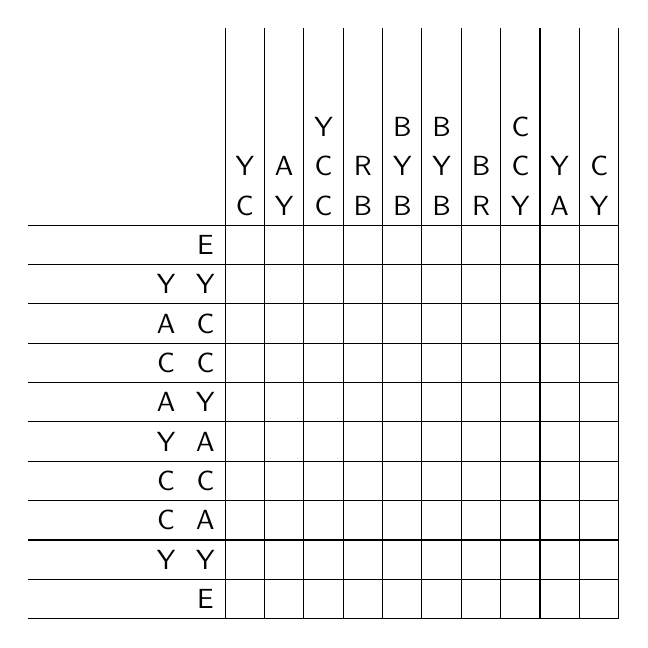
\begin{tikzpicture}[scale=0.5]
%\node at (-2.5,12.5) {Cancer};
   
    \foreach \n in {0,...,10}{
        \draw (-5,\n)--(10,\n);
        \draw (\n,0)--(\n,15);
    }
   
    %Horizontal Clues (backwards in source)
    \foreach[count=\n] \x in {E}{\node at ({0.5-\n},9.5) {\nonosize{\x}}; }
    \foreach[count=\n] \x in {Y,Y}{\node at ({0.5-\n},8.5) {\nonosize{\x}}; }
    \foreach[count=\n] \x in {C,A}{\node at ({0.5-\n},7.5) {\nonosize{\x}}; }
    \foreach[count=\n] \x in {C,C}{\node at ({0.5-\n},6.5) {\nonosize{\x}}; }
    \foreach[count=\n] \x in {Y,A}{\node at ({0.5-\n},5.5) {\nonosize{\x}}; }
    \foreach[count=\n] \x in {A,Y}{\node at ({0.5-\n},4.5) {\nonosize{\x}}; }
    \foreach[count=\n] \x in {C,C}{\node at ({0.5-\n},3.5) {\nonosize{\x}}; }
    \foreach[count=\n] \x in {A,C}{\node at ({0.5-\n},2.5) {\nonosize{\x}}; }
    \foreach[count=\n] \x in {Y,Y}{\node at ({0.5-\n},1.5) {\nonosize{\x}}; }
    \foreach[count=\n] \x in {E}{\node at ({0.5-\n},0.5) {\nonosize{\x}}; }
   
    %Vertical Clues (backwards in source)
    \foreach[count=\n] \x in {C,Y}{\node at (0.5,{9.5+\n}) {\nonosize{\x}}; }
    \foreach[count=\n] \x in {Y,A}{\node at (1.5,{9.5+\n}) {\nonosize{\x}}; }
    \foreach[count=\n] \x in {C,C,Y}{\node at (2.5,{9.5+\n}) {\nonosize{\x}}; }
    \foreach[count=\n] \x in {B,R}{\node at (3.5,{9.5+\n}) {\nonosize{\x}}; }
    \foreach[count=\n] \x in {B,Y,B}{\node at (4.5,{9.5+\n}) {\nonosize{\x}}; }
    \foreach[count=\n] \x in {B,Y,B}{\node at (5.5,{9.5+\n}) {\nonosize{\x}}; }
    \foreach[count=\n] \x in {R,B}{\node at (6.5,{9.5+\n}) {\nonosize{\x}}; }
    \foreach[count=\n] \x in {Y,C,C}{\node at (7.5,{9.5+\n}) {\nonosize{\x}}; }
    \foreach[count=\n] \x in {A,Y}{\node at (8.5,{9.5+\n}) {\nonosize{\x}}; }
    \foreach[count=\n] \x in {Y,C}{\node at (9.5,{9.5+\n}) {\nonosize{\x}}; }
\end{tikzpicture}
\end{center}

\vfill

% \begin{center}
% \begin{tikzpicture}[scale=0.5]
   
%     \foreach \n in {0,...,8}{
%         \draw (-5,\n)--(10,\n);
%         \draw (\n,0)--(\n,8);
%     }
%     \foreach \n in {9,10}{
%         \draw (\n,0)--(\n,8);
%     }
   
%     %Horizontal Clues (backwards in source)
%     \foreach[count=\n] \x in {MP 1}{\node at ({-\n},7.5) {\nonosize{\x}}; }
%     \foreach[count=\n] \x in {MP 1}{\node at ({-\n},6.5) {\nonosize{\x}}; }
%     \foreach[count=\n] \x in {MP 3}{\node at ({-\n},5.5) {\nonosize{\x}}; }
%     \foreach[count=\n] \x in {MP 4}{\node at ({-\n},4.5) {\nonosize{\x}}; }
%     \foreach[count=\n] \x in {CP 1}{\node at ({-\n},3.5) {\nonosize{\x}}; }
%     \foreach[count=\n] \x in {CP 2}{\node at ({-\n},2.5) {\nonosize{\x}}; }
%     \foreach[count=\n] \x in {CP 3}{\node at ({-\n},1.5) {\nonosize{\x}}; }
%     \foreach[count=\n] \x in {CP 4}{\node at ({-\n},0.5) {\nonosize{\x}}; }

%     %Alicorn c == 2
%     {2}{\node at (3.5,7.5) {\nonosize{\textcolor{black!20}2}}; }
%     %Mantichore a == 5
%     {5}{\node at (1.5,6.5) {\nonosize{\textcolor{black!20}5}}; }
%     %Quinotar n == 0 and r == 6
%     {6}{\node at (3.5,5.5) {\nonosize{\textcolor{black!20}6}}; }
%     {0}{\node at (7.5,5.5) {\nonosize{\textcolor{black!20}0}}; }
%     %Chimera e == 7
%     {7}{\node at (4.5,4.5) {\nonosize{\textcolor{black!20}7}}; }
%     %Myrmidon y == 3
%     {3}{\node at (1.5,3.5) {\nonosize{\textcolor{black!20}3}}; }
%     %Drakaina d == 4
%     {4}{\node at (0.5,2.5) {\nonosize{\textcolor{black!20}4}}; }
%     %Hobgoblin b == 1
%     {1}{\node at (2.5,1.5) {\nonosize{\textcolor{black!20}1}}; }
%     %Wyvern w == 8
%     {8}{\node at (0.5,0.5) {\nonosize{\textcolor{black!20}8}}; }

% \end{tikzpicture}

\begin{center}
\(0\) is MP1's fourth. \(1\) is CP1's third.
\(2\) is MP3's first. \(3\) is CP3's second.
\(4\) is CP2's first.
\end{center}
\begin{center}
\(5\) is MP2's second.
\(6\) is MP1's last. \(7\) is MP3's fifth.
\(8\) is CP3's first. There is no \(9\).
\end{center}


\vfill

\newpage



\puzzleTitle{Our Twelve Signs}

\vfill
\begin{center}
$\arraycolsep=1cm
\begin{array}{c c c}
\vspace*{1cm}
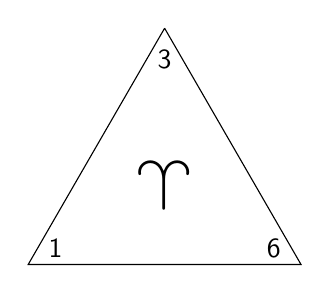
\begin{tikzpicture}
\draw (90:2) -- (-150:2) -- (-30:2) -- (90:2);
{\Huge \node at (0,0) {\aries};}
\node at (-150:1.6) {1};
\node at (-30:1.6) {6};
\node at (90:1.6) {3};
\end{tikzpicture}
&
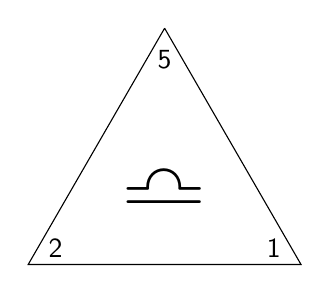
\begin{tikzpicture}
\draw (90:2) -- (-150:2) -- (-30:2) -- (90:2);
{\Huge \node at (0,0) {\libra};}
\node at (-150:1.6) {2};
\node at (-30:1.6) {1};
\node at (90:1.6) {5};
\end{tikzpicture}
&

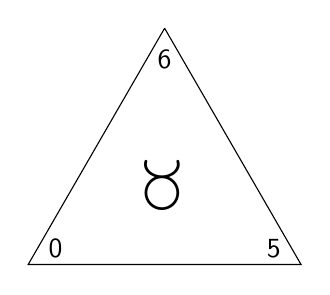
\begin{tikzpicture}
\draw (90:2) -- (-150:2) -- (-30:2) -- (90:2);
{\Huge \node at (0,0) {\taurus};}
\node at (-150:1.6) {0};
\node at (-30:1.6) {5};
\node at (90:1.6) {6};
\end{tikzpicture}\\
\vspace*{1cm}

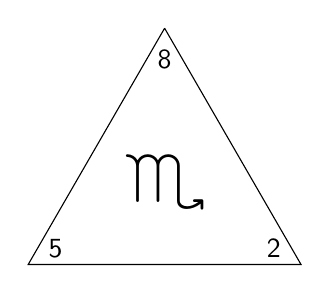
\begin{tikzpicture}
\draw (90:2) -- (-150:2) -- (-30:2) -- (90:2);
{\Huge \node at (0,0) {\scorpio};}
\node at (-150:1.6) {5};
\node at (-30:1.6) {2};
\node at (90:1.6) {8};
\end{tikzpicture}
&

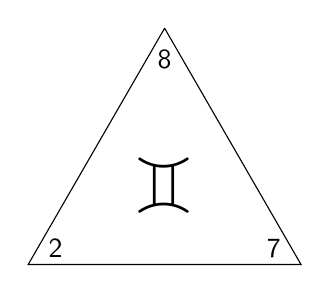
\begin{tikzpicture}
\draw (90:2) -- (-150:2) -- (-30:2) -- (90:2);
{\Huge \node at (0,0) {\gemini};}
\node at (-150:1.6) {2};
\node at (-30:1.6) {7};
\node at (90:1.6) {8};
\end{tikzpicture}
&
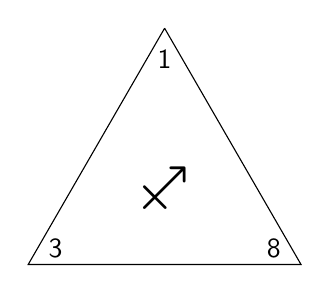
\begin{tikzpicture}
\draw (90:2) -- (-150:2) -- (-30:2) -- (90:2);
{\Huge \node at (0,0) {\sagittarius};}
\node at (-150:1.6) {3};
\node at (-30:1.6) {8};
\node at (90:1.6) {1};
\end{tikzpicture}\\
\vspace*{1cm}
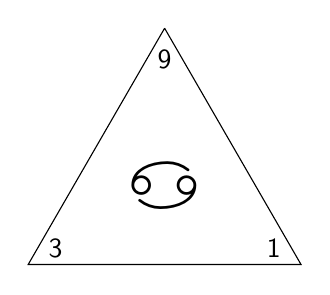
\begin{tikzpicture}
\draw (90:2) -- (-150:2) -- (-30:2) -- (90:2);
{\Huge \node at (0,0) {\cancer};}
\node at (-150:1.6) {3};
\node at (-30:1.6) {1};
\node at (90:1.6) {9};
\end{tikzpicture}
&
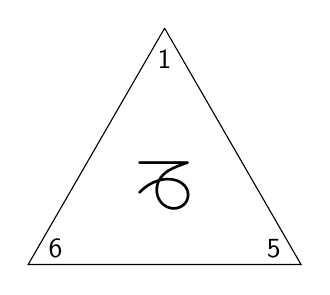
\begin{tikzpicture}
\draw (90:2) -- (-150:2) -- (-30:2) -- (90:2);
{\Huge \node at (0,0) {\capricornus};}
\node at (-150:1.6) {6};
\node at (-30:1.6) {5};
\node at (90:1.6) {1};
\end{tikzpicture}
&

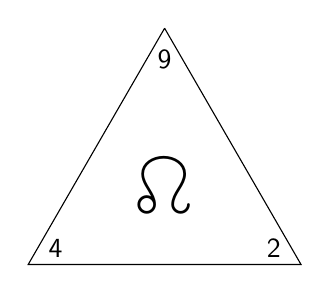
\begin{tikzpicture}
\draw (90:2) -- (-150:2) -- (-30:2) -- (90:2);
{\Huge \node at (0,0) {\leo};}
\node at (-150:1.6) {4};
\node at (-30:1.6) {2};
\node at (90:1.6) {9};
\end{tikzpicture}\\
\vspace*{1cm}
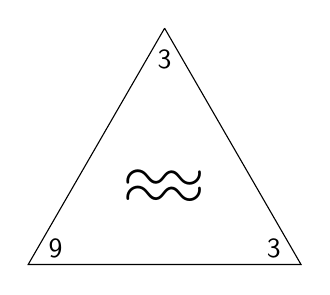
\begin{tikzpicture}
\draw (90:2) -- (-150:2) -- (-30:2) -- (90:2);
{\Huge \node at (0,0) {\aquarius};}
\node at (-150:1.6) {9};
\node at (-30:1.6) {3};
\node at (90:1.6) {3};
\end{tikzpicture}
&

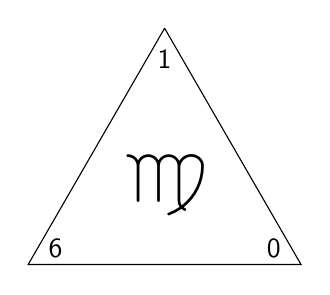
\begin{tikzpicture}
\draw (90:2) -- (-150:2) -- (-30:2) -- (90:2);
{\Huge \node at (0,0) {\virgo};}
\node at (-150:1.6) {6};
\node at (-30:1.6) {0};
\node at (90:1.6) {1};
\end{tikzpicture}
&
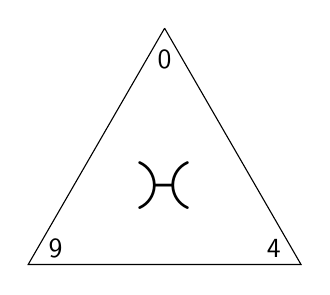
\begin{tikzpicture}
\draw (90:2) -- (-150:2) -- (-30:2) -- (90:2);
{\Huge \node at (0,0) {\pisces};}
\node at (-150:1.6) {9};
\node at (-30:1.6) {4};
\node at (90:1.6) {0};
\end{tikzpicture}
\end{array}$
\end{center}
\vfill

\newpage


\puzzleTitle{Code Reference}

\vfill

\begin{multicols}{2}
\begin{center}\small
  \begin{tabular}{c|c|c|c|c}
    \footnotesize
    Letter &
    \footnotesize
      Decimal &
    \footnotesize
      Binary &
    \footnotesize
      Morse &
    \footnotesize
      Braille \\\hline
%    \footnotesize
%      ROT13\\\hline
    A &
      1 &
      00001 &
      \morseDit\morseDah &
      \braille{a}\\
%      N\\
    B &
      2 &
      00010 &
      \morseDah\morseDit\morseDit\morseDit &
      \braille{b}\\
%      O\\
    C &
      3 &
      00011 &
      \morseDah\morseDit\morseDah\morseDit &
      \braille{c}\\
%      P\\
    D &
      4 &
      00100 &
      \morseDah\morseDit\morseDit &
      \braille{d}\\
%      Q\\
    E &
      5 &
      00101 &
      \morseDit &
      \braille{e}\\
%      R\\
    F &
      6 &
      00110 &
      \morseDit\morseDit\morseDah\morseDit &
      \braille{f}\\
%      S\\
    G &
      7 &
      00111 &
      \morseDah\morseDah\morseDit &
      \braille{g}\\
%      T\\
    H &
      8 &
      01000 &
      \morseDit\morseDit\morseDit\morseDit &
      \braille{h}\\
%      U\\
    I &
      9 &
      01001 &
      \morseDit\morseDit &
      \braille{i}\\
%      V\\
    J &
      10 &
      01010 &
      \morseDit\morseDah\morseDah\morseDah &
      \braille{j}\\
%      W\\
    K &
      11 &
      01011 &
      \morseDah\morseDit\morseDah &
      \braille{k}\\
%      X\\
    L &
      12 &
      01100 &
      \morseDit\morseDah\morseDit\morseDit &
      \braille{l}\\
%      Y\\
    M &
      13 &
      01101 &
      \morseDah\morseDah &
      \braille{m}\\
%      Z\\
  \end{tabular}

  \begin{tabular}{c|c|c|c|c}
    \footnotesize
    Letter &
    \footnotesize
      Decimal &
    \footnotesize
      Binary &
    \footnotesize
      Morse &
    \footnotesize
      Braille \\\hline
%    \footnotesize
%      ROT13\\\hline
    N &
      14 &
      01110 &
      \morseDah\morseDit &
      \braille{n}\\
%      A\\
    O &
      15 &
      01111 &
      \morseDah\morseDah\morseDah &
      \braille{o}\\
%      B\\
    P &
      16 &
      10000 &
      \morseDit\morseDah\morseDah\morseDit &
      \braille{p}\\
%      C\\
    Q &
      17 &
      10001 &
      \morseDah\morseDah\morseDit\morseDah &
      \braille{q}\\
%      D\\
    R &
      18 &
      10010 &
      \morseDit\morseDah\morseDit &
      \braille{r}\\
%      E\\
    S &
      19 &
      10011 &
      \morseDit\morseDit\morseDit &
      \braille{s}\\
%      F\\
    T &
      20 &
      10100 &
      \morseDah &
      \braille{t}\\
%      G\\
    U &
      21 &
      10101 &
      \morseDit\morseDit\morseDah &
      \braille{u}\\
%      H\\
    V &
      22 &
      10110 &
      \morseDit\morseDit\morseDit\morseDah &
      \braille{v}\\
%      I\\
    W &
      23 &
      10111 &
      \morseDit\morseDah\morseDah &
      \braille{w}\\
%      J\\
    X &
      24 &
      11000 &
      \morseDah\morseDit\morseDit\morseDah &
      \braille{x}\\
%      K\\
    Y &
      25 &
      11001 &
      \morseDah\morseDit\morseDah\morseDah &
      \braille{y}\\
%      L\\
    Z &
      26 &
      11010 &
      \morseDah\morseDah\morseDit\morseDit &
      \braille{z}\\
%      M\\
  \end{tabular}
\end{center}
\end{multicols}

\vfill

\newpage

\lfoot{\thepage/\pageref*{LastPage} (Organizer Appendix)}

\puzzleTitle{Clues}
\clue{
Main Puzzle 1

To succeed at an institution like Rudin Academy, you must not only forge strong friendships, but you must also study under the appropriate mentors. But of course, it is not so easy that they would just tell you which mentors you are paired with. To find the appropriate mentors, everything must be in absolute balance. Below are pictures of several potential mentoring programs and hidden in these programs is a "magic word" to be deciphered.

The dots in the pictures represent the people (both students and mentors). Lines are connected between pairs of dots if they have a mentor/mentee relationship. Many of the lines are labeled with numbers already. Each person has a value equal to the sum of the labels of each connection (line) that person has. For instance, the person shown below has the value `16' because the lines incident to this person have labels 1,4, and 11.

\vspace*{1cm}

\begin{center}
\begin{tikzpicture}[scale=1.5]
\draw [dashed] (0,0)--(1,0);
\draw [dashed] (2,2)--(2,1);
\draw [dashed] (3,0)--(4,0);
\draw (1,0)--(3,0);
\draw (2,1)--(2,0);

\draw[fill=black] (2,0) circle (0.075);

{\Large
\node at (1.25,.2) {$1$};
\node at (2.20,.75) {$4$};
\node at (2.75,.2) {$11$};
\node at (2,-.25) {$16$};
}
\end{tikzpicture}

\end{center}

In an ideal mentoring program, every person has the \textbf{same} value. (However, two people in different mentoring programs may or may not have the same value.)

Also, we are restricted with what numbers we can use to label the lines! In the first picture we can only use the integers $\left\{1,2, \ldots,9\right\}$ and each integer is only used once. In the second picture we can only use the integers $\left\{1,2, \ldots,16\right\}$ and each integer is only used once. For the third picture, we can use unique integers from the set $\left\{1, 2, \ldots, 12 \right\}$ but now we notice that not all of these integers may be used! 

}

\newpage

\clue{
Main Puzzle 2

Attending a private school of magic ain't cheap, and I'm pretty sure
they make the tuition schedule complicated on purpose. In fact,
I think the accountant in charge of billing is one of those evil
"Death Drinkers" you may have heard about.

It seems what I'm supposed to do is fill out the \(10\times10\) grid
using the digits \(0\) through \(9\). It's kind of like a Sudoku:
each digit should appear exactly once in every row and column, and also
exactly once in every \(2\times 5\) subrectangle marked by bold
borders the background shading. I've completed a \(6\times 6\) example
using \(2\times 3\) subrectangles below to give you the idea.

What's especially evil is that I don't think the grid is uniquely
solvable: there's gonna be some cells that you just don't have enough
information to figure out. But that's okay: if you use the
letters in the corners of cells that you are able to determine, you'll be able
to spell out one of Rudin Academy's magic words.

\begin{center}
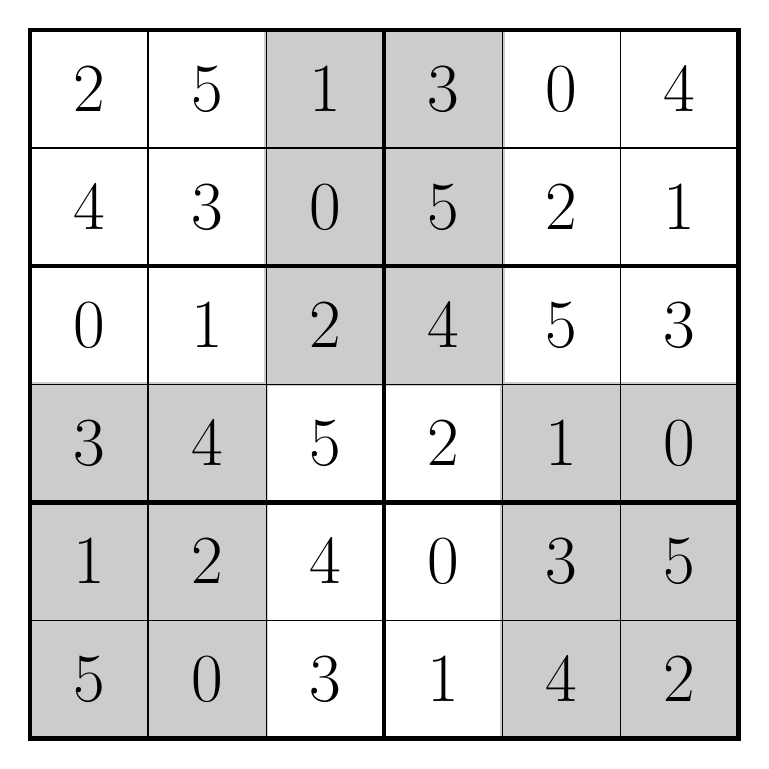
\begin{tikzpicture}[scale=1.5]
\draw[fill=black!05,ultra thick,color=black!20](0,0) rectangle (2,3);
\draw[fill=black!05,ultra thick,color=black!20](2,3) rectangle (4,6);
\draw[fill=black!05,ultra thick,color=black!20](4,0) rectangle (6,3);
\draw[ultra thick](0,0) rectangle (6,6);

 
\draw(0,0)grid(6,6);
%\draw(3,0)grid(3,10);
%\draw(5,0)grid(5,10);
%\draw(7,0)grid(7,10);
%\draw(9,0)grid(9,10);
% 
%\draw(0,1)grid(10,1);
%\draw(0,3)grid(10,3);
%% \draw(0,5)grid(10,5);
%\draw(0,7)grid(10,7);
%\draw(0,9)grid(10,9);
 
\draw[ultra thick](0,0)rectangle(3,2);
\draw[ultra thick](0,2)rectangle(3,4);
\draw[ultra thick](0,4)rectangle(3,6);
\draw[ultra thick](3,0)rectangle(6,2);
\draw[ultra thick](3,2)rectangle(6,4);
\draw[ultra thick](3,4)rectangle(6,6);
 
%\draw[loosely dashed](2,0)grid(2,10);
%\draw[loosely dashed](4,0) to (4,10);
%\draw[loosely dashed](6,0)grid(6,10);
%\draw[loosely dashed](8,0)grid(8,10);
%\draw[loosely dashed](0,5) to (10,5);
 
 {\Huge
\foreach\x[count=\i] in{2,5,1,3,0,4 }{\node at(\i-0.5,5.5){$\x$};};
\foreach\x[count=\i] in{4,3,0,5,2,1 }{\node at(\i-0.5,4.5){$\x$};};
\foreach\x[count=\i] in{0,1,2,4,5,3 }{\node at(\i-0.5,3.5){$\x$};};
\foreach\x[count=\i] in{3,4,5,2,1,0 }{\node at(\i-0.5,2.5){$\x$};};
\foreach\x[count=\i] in{1,2,4,0,3,5 }{\node at(\i-0.5,1.5){$\x$};};
\foreach\x[count=\i] in{5,0,3,1,4,2 }{\node at(\i-0.5,0.5){$\x$};};
}
\end{tikzpicture}\end{center}
}

\newpage


\clue{
Main Puzzle 3

The class I'm most excited to take is "Defense Against the Scary Spells".
The curriculum found in my welcome packet includes four of the basic
shield spells. Their
names are basically nonsense, and it looks like the packet is missing a few letters as well.
That said, if you can match each shield boundary with the graph equation that matches
it below, you'll be able to figure them out.

What I've yet to learn is how to choose a shield to use against each attack.
Attacks are infinitely-many points in the plane with vertical
coordinates that increase to \(\infty\). If the shield covers all
except a finite number of the attack points, it's successful, but if the shield fails
to cover infinitely-many of the attack points' it's defeated.

There's got to be a way to use the shield names to spell out one of Rudin Academy's
magic words.

\[\texttt{\_A\_U\_U\_}
\hspace{2em} y=|x|-2\]
\[\texttt{\_I\_A\_U\_} \hspace{2em}
y=\frac{5x^2-4}{x^2+1}\]
\[\texttt{\_A\_E\_R\_}\hspace{2em}
  y=\begin{cases}
    x^2 & \text{ if }x\text{ is an integer} \\
    -3 & \text{otherwise}
    \end{cases}
\]
\[\texttt{\_O\_F\_I\_}\hspace{2em}
y=\frac{1}{|x|}\hspace{1em}(x\not=0)\]

\begin{enumerate}[I]
\item Shield defeated by \(\{(\frac{1}{2}-n,n-\frac{9}{2}):n\in\mathbb Z^+\}
  =\{(-\frac{1}{2},-\frac{7}{2}),(-\frac{3}{2},-\frac{5}{2}),(-\frac{5}{2},-\frac{3}{2}),\dots\}\)
\item Shield defeated by \(\{(\frac{n^2+1}{n},\sqrt{n}):n\in\mathbb Z^+\}\)
\item Shield defeated by \(\{(0,n^2-10):n\in\mathbb Z^+\}\)
\item Shield defeated by \(\{(n-3,2n):n\in\mathbb Z^+\}\)
\item Shield defeated by \(\{(\frac{4}{n^2},\frac{n}{2}):n\in\mathbb Z^+\}\)
\item Shield defeated by \(\{(-1)^nn,n+5):n\in\mathbb Z^+\}\)
\item Cannot be defeated by any attack with vertical coordinates increasing
  toward \(\infty\).
\end{enumerate}

}

\newpage



\clue{
Cryptic Puzzle 1

At Rudin Academy, Arithmancy is taught by a team of three professors: one who wields a wand in their left hand, one who wields a wand in their right hand, and one who wields one wand in each hand at the same time. While arithmancy problems look like the arithmetic you are used to in non-magical school, each magician computes their solutions in a unique way.

I'm told that each of these professors wrote three exercises for the school's placement exam. I expect that a magic word can be revealed by matching the nine provided solutions from the answer bank to each exercise, once you make a slight adjustment based on the nature of each exercise’s author.

}
\newpage


\clue{
Cryptic Puzzle 2

Rudin Academy is well-known for its Astronomy course, which uses patterns in
the night sky to provide cryptic predictions about the days to come.

``Our Night Sky'' in the welcome packet is an example of such a divination.
Hidden among the one hundred letters in this square are twenty ``stars'' that
spell out a message. The location
of these stars may be divined by considering the following four rules:

\begin{itemize}
\item Exactly two stars appear in each horizontal row.
\item Exactly two stars appear in each vertical column.
\item Exactly two stars appear in each shape within the square.
\item No star ever appears directly next to another star (vertically, horizontally,
      or diagonally), as illustrated below.
\end{itemize}

Not only does this message answer the question ``When did the magician know he
had discovered something special?'', but it also contains one of the academy's
magic words.

\begin{center}\Large
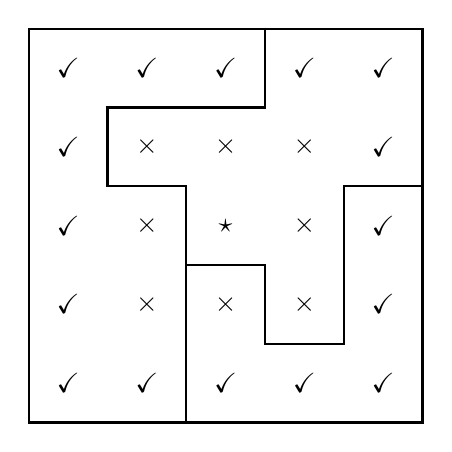
\begin{tikzpicture}
\draw[thick] (0,0) rectangle (5,5);
\draw[thick] (2,0) -- (2,3) -- (1,3) -- (1,4) -- (3,4) -- (3,5);
\draw[thick] (2,2) -- (3,2) -- (3,1) -- (4,1) -- (4,3) -- (5,3);
\foreach\x[count=\i from 0] in {\checkmark,\checkmark,\checkmark,\checkmark,\checkmark}{\node at(\i.5,4.5){\x};};
\foreach\x[count=\i from 0] in {\checkmark,$\times$,$\times$,$\times$,\checkmark}{\node at(\i.5,3.5){\x};};
\foreach\x[count=\i from 0] in {\checkmark,$\times$,$\star$,$\times$,\checkmark}{\node at(\i.5,2.5){\x};};
\foreach\x[count=\i from 0] in {\checkmark,$\times$,$\times$,$\times$,\checkmark}{\node at(\i.5,1.5){\x};};
\foreach\x[count=\i from 0] in {\checkmark,\checkmark,\checkmark,\checkmark,\checkmark}{\node at(\i.5,0.5){\x};};
\end{tikzpicture}
\end{center}
}

\newpage



\clue{
Cryptic Puzzle 3

Like yourselves, magicians observe a 365 day year, except that every fourth year (a “leap year”) must include a 366th day. Likewise, their weeks generally include seven days, Monday through Sunday. But the magical calendar uses 13 months rather than the usual 12: Jan, Feb, Mar, Apr, May, Jun, Sol, Jul, Aug, Sep, Oct, Nov, and Dec. This allows each month to include 28 days, a sensible pattern which guarantees that the 1st of each month is always a Monday, and the 28th is always a Sunday.

Ah you say, but that only adds up to 364 days a year? Very good! So to account for this, a 29th day, called Magday, occurs on December 29 every year, and on June 29 every leap year. As the name might suggest, magical powers are particularly powerful on Magday.

Knowing this will be important to help me plan my schedule. I have to complete six special courses throughout my time at the Academy. Each special course lasts a specific number of days, and is designed so that a specific day of the course must be a Magday. Additionally, each such course must begin on the day immediately following the end of the previous course: for example, if a course ends on Sol 28, the next course must begin on Jul 1. Also, these courses require a lot of work, so no skipping weekends or any other day.

I get the feeling that there's really only one way I can make this work, and if you can
help me figure it out, you'll find yet another magic word.
}

\newpage



\clue{
Metapuzzle

Thanks for all your help revealing the school's magic words for me, but it's about
time to uncover the most magical word of all. My guess is that the regular magic words
need to be combined to create a spell that will reveal the school's Seal.
The only other clues I have for you are the images below...


\begin{center}
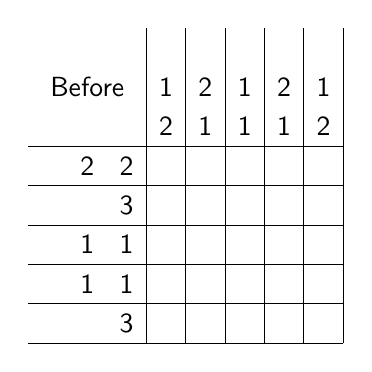
\begin{tikzpicture}[scale=0.5]
\node at (-1.5,6.5) {Before};
   
    \foreach \n in {0,...,5}{
        \draw (-3,\n)--(5,\n);
        \draw (\n,0)--(\n,8);
    }
   
    %Horizontal Clues (backwards in source)
    \foreach[count=\n] \x in {2,2}{\node at ({0.5-\n},4.5) {\nonosize{\x}}; }
    \foreach[count=\n] \x in {3}{\node at ({0.5-\n},3.5) {\nonosize{\x}}; }
    \foreach[count=\n] \x in {1,1}{\node at ({0.5-\n},2.5) {\nonosize{\x}}; }
    \foreach[count=\n] \x in {1,1}{\node at ({0.5-\n},1.5) {\nonosize{\x}}; }
    \foreach[count=\n] \x in {3}{\node at ({0.5-\n},0.5) {\nonosize{\x}}; }
   
    %Vertical Clues (backwards in source)
    \foreach[count=\n] \x in {2,1}{\node at (0.5,{4.5+\n}) {\nonosize{\x}}; }
    \foreach[count=\n] \x in {1,2}{\node at (1.5,{4.5+\n}) {\nonosize{\x}}; }
    \foreach[count=\n] \x in {1,1}{\node at (2.5,{4.5+\n}) {\nonosize{\x}}; }
    \foreach[count=\n] \x in {1,2}{\node at (3.5,{4.5+\n}) {\nonosize{\x}}; }
    \foreach[count=\n] \x in {2,1}{\node at (4.5,{4.5+\n}) {\nonosize{\x}}; }
\end{tikzpicture}
\hspace{3em}
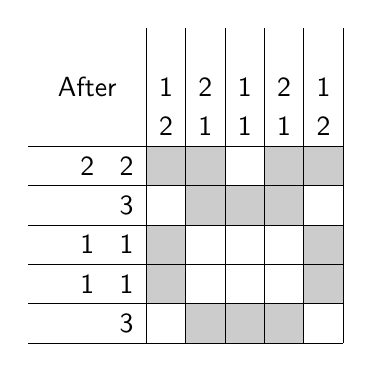
\begin{tikzpicture}[scale=0.5]
\node at (-1.5,6.5) {After};
   
    \fill[color=black!20] (1,0) rectangle (4,1);
    \fill[color=black!20] (0,1) rectangle (1,3);
    \fill[color=black!20] (4,1) rectangle (5,3);
    \fill[color=black!20] (4,1) rectangle (5,3);
    \fill[color=black!20] (1,3) rectangle (4,4);
    \fill[color=black!20] (0,4) rectangle (2,5);
    \fill[color=black!20] (3,4) rectangle (5,5);
    \foreach \n in {0,...,5}{
        \draw (-3,\n)--(5,\n);
        \draw (\n,0)--(\n,8);
    }
   
    %Horizontal Clues (backwards in source)
    \foreach[count=\n] \x in {2,2}{\node at ({0.5-\n},4.5) {\nonosize{\x}}; }
    \foreach[count=\n] \x in {3}{\node at ({0.5-\n},3.5) {\nonosize{\x}}; }
    \foreach[count=\n] \x in {1,1}{\node at ({0.5-\n},2.5) {\nonosize{\x}}; }
    \foreach[count=\n] \x in {1,1}{\node at ({0.5-\n},1.5) {\nonosize{\x}}; }
    \foreach[count=\n] \x in {3}{\node at ({0.5-\n},0.5) {\nonosize{\x}}; }
   
    %Vertical Clues (backwards in source)
    \foreach[count=\n] \x in {2,1}{\node at (0.5,{4.5+\n}) {\nonosize{\x}}; }
    \foreach[count=\n] \x in {1,2}{\node at (1.5,{4.5+\n}) {\nonosize{\x}}; }
    \foreach[count=\n] \x in {1,1}{\node at (2.5,{4.5+\n}) {\nonosize{\x}}; }
    \foreach[count=\n] \x in {1,2}{\node at (3.5,{4.5+\n}) {\nonosize{\x}}; }
    \foreach[count=\n] \x in {2,1}{\node at (4.5,{4.5+\n}) {\nonosize{\x}}; }
\end{tikzpicture}

\vspace{2em}

{\Huge \(\gamma\), \(\varepsilon\), \(\beta\), \(\delta-30\), \(\alpha+3\), \(\zeta-5\)}

\end{center}
}


\newpage


\clue{
Bonus Puzzle

Hey, it looks like you're pretty good at this Rune stuff, huh? For a few bonus
points, maybe you can help me use all twelve unique Signs to
design four Runes, such that as many of the following
two-digit numbers are used for \(\delta\), \(\varepsilon\), and \(\zeta\) as possible:

\begin{itemize}
\item \(02\)
\item \(03\)
\item \(12\)
\item \(13\)
\item \(26\)
\item \(30\)
\item \(34\)
\item \(41\)
\item \(59\)
\item \(79\)
\item \(81\)
\item \(83\)
\end{itemize}
% one perfect solution:
% 933, 065, 492
% 904, 251, 136
% 610, 287, 391
% 582, 318, 615

Bring your ClueKeeper app to the location designated by your game's organizers
to score your solution. If you do, you'll earn \(N-4\) points,
where \(N\) counts how many of the above twelve numbers are included in your four Runes
(making this puzzle worth a maximum of \(8\) points).
}

\newpage



\clue{
Unlocking puzzles (instructions/illustration omitted in ClueKeeper for Cryptic Puzzle unlocks)

To unlock this puzzle, we'll first need to determine its magic code, a three-digit number.
A magic code is obtained by combining three of the school's twelve Signs from the welcome
packet into the configuration illustrated below. Then the code is given by the Greek
letters \(\alpha\beta\gamma\); for the example below, the magic code would be \(123\).

In the example below, we also have \(\delta=45\), \(\varepsilon=67\), and \(\zeta=89\).
For this puzzle's magic code, you'll need to find the only combination of Signs
that satisfies the following requirements:

\begin{itemize}
\item \(\delta\) VARIES
\item \(\varepsilon\) VARIES
\item \(\zeta\) VARIES
\end{itemize}

Once you've figured out the magic code \(\alpha\beta\gamma\),
submit it in the ClueKeeper app to unlock this
puzzle. (If your game is using ClueKeeper's GPS feature, you'll need to be at the
location corresponding to this code given on your Campus Map to submit it.)


\begin{center}
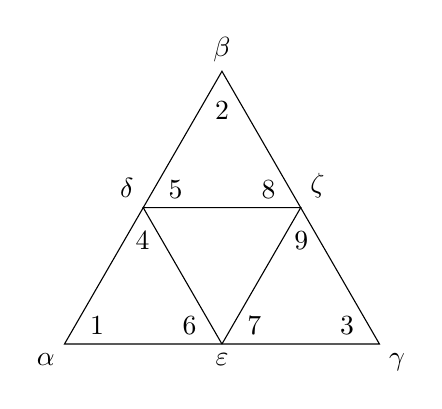
\begin{tikzpicture}
    \draw (0:0) -- (0:2) -- (90:3.4641) -- (180:2) -- (0,0);
    \draw (0:0) -- (60:2) -- (120:2) -- (0:0);

    \node[anchor=north east] at (180:2) {\(\alpha\)};
    \node[anchor=south] at (90:3.4641) {\(\beta\)};
    \node[anchor=north west] at (0:2) {\(\gamma\)};
    \node[anchor=south east] at (120:2) {\(\delta\)};
    \node[anchor=north] at (0:0) {\(\varepsilon\)};
    \node[anchor=south west] at (60:2) {\(\zeta\)};

    \node[anchor=south west] at (180:1.8) {\(1\)};
    \node[anchor=north] at (90:3.2) {\(2\)};
    \node[anchor=south east] at (0:1.8) {\(3\)};
    \node[anchor=north] at (123:1.85) {\(4\)};
    \node[anchor=south west] at (115:1.9) {\(5\)};
    \node[anchor=south east] at (180:0.2) {\(6\)};
    \node[anchor=south west] at (0:0.2) {\(7\)};
    \node[anchor=south east] at (65:1.9) {\(8\)};
    \node[anchor=north] at (57:1.85) {\(9\)};
\end{tikzpicture}
\end{center}
}

\newpage

\clue{
Unlocking puzzle clues

Main Puzzle 1
\begin{itemize}
\item \(\delta\): pentagonal number
\item \(\varepsilon\): digits sum to \(10\)
\item \(\zeta\): digits sum to \(4\)
\end{itemize}

Main Puzzle 2
\begin{itemize}
\item \(\delta\): abundant, and digits sum to \(15\)
\item \(\varepsilon\): digits sum to \(3\)
\item \(\zeta\): prime larger than \(10\)
\end{itemize}

Main Puzzle 3
\begin{itemize}
\item \(\delta\): twin prime
\item \(\varepsilon\): least whole number
\item \(\zeta\): two less than a multiple of \(11\)
\end{itemize}

Cryptic Puzzle 1
\begin{itemize}
\item \(\delta\): twin prime
\item \(\varepsilon\): prime less than \(10\)
\item \(\zeta\): prime but not a twin prime
\end{itemize}

Cryptic Puzzle 2
\begin{itemize}
\item \(\delta\): even
\item \(\varepsilon\): digits sum to \(14\)
\item \(\zeta\): multiple of \(\delta\)
\end{itemize}

Cryptic Puzzle 3
\begin{itemize}
\item \(\delta\): used as \(\delta\), \(\varepsilon\) or \(\zeta\) for Cryptic Puzzle 1
\item \(\varepsilon\): sum of six consecutive primes
\item \(\zeta\): pentagonal number
\end{itemize}
}

\newpage

\clue{
Hidden Puzzle

Have you noticed the ``fantastic'' connection between all the magic words?
}

\newpage

\puzzleTitle{Solutions}

\begin{itemize}
\item Main Puzzle 1 [RUNE]: 353
\item Main Puzzle 1: QUINOTAUR
\item Cryptic Puzzle 1 [RUNE]: 611
\item Cryptic Puzzle 1: HOBGOBLIN
\item Main Puzzle 2 [RUNE]: 416
\item Main Puzzle 2: MANTICHORE
\item Cryptic Puzzle 2 [RUNE]: 664
\item Cryptic Puzzle 2: DRAKAINA
\item Main Puzzle 3 [RUNE]: 615
\item Main Puzzle 3: CHIMERA
\item Cryptic Puzzle 3 [RUNE]: 231
\item Cryptic Puzzle 3: WYVERN
\item Metapuzzle: AMAZED
\item Hidden Puzzle: FANTASTIC BEASTS
\end{itemize}


\end{document}
